\documentclass{article}
\usepackage[utf8]{inputenc}
\usepackage[english,ngerman]{babel}
%% ========================================================================
%%%% MISC usepackages
%% ========================================================================

%% Chemistry
\usepackage{chemfig,chemmacros}
\usepackage{bohr}
\usepackage{elements}
\chemsetup{modules = all}
\chemsetup[redox]{explicit-sign = true}
\chemsetup[phases]{pos=sub}
%\chemsetup[reactions]{before-tag = {R}, tag-open = [, tag-close = ]}
  
%% Maths
\usepackage{amsmath,amssymb,amsthm,textcomp}

%% Physics
\usepackage{siunitx}

%% Graphics
\usepackage{graphicx}
\usepackage{tikz}
\usepackage{rotating}
%\usepackage{subfig}

%% Tables and Lists
\usepackage{enumerate}
\usepackage{multicol}
\usepackage{geometry}
\usepackage{tabu}
\usepackage{listings}
\usepackage{tabularx}

%% Structures and Style
\usepackage{caption}
\usepackage{subcaption}
\usepackage{booktabs}
\usepackage{colortbl}

\usepackage{xcolor}
\usepackage{xfrac}
\usepackage[export]{adjustbox}[2011/08/13]

\usepackage{booktabs}
\usepackage{float}

\usepackage{fancyhdr}

%% Citing and Settings
\usepackage[backend=biber,
style=numeric,
backref=true, 
natbib=true, %% offering natbib-compatible commands
hyperref=true, %% using hyperref-package references
sorting= none,
doi=true,
maxcitenames=10,
maxbibnames=100,
citestyle=numeric
]{biblatex}

\addbibresource{references.bib}

\usepackage[toc,automake]{glossaries}
\include{abbrevations}
\makeglossaries

\usepackage[colorlinks=true,linkcolor=blue]{hyperref}

%% Figure settings
\renewcommand{\figurename}{Abbildung}
\renewcommand{\tablename}{Tabelle}
\renewcommand{\listfigurename}{Abbildungsverzeichnis}
\renewcommand{\listtablename}{Tabellenverzeichnis}

%% Commands chemistry

\NewChemState\ElPot{ symbol=E , subscript-pos=right , superscript= , unit=\volt}

%% ========================================================================
%%%% Document Information
%% ========================================================================

%% Title 
\title{Herstellung von \ch{CuSO4 * 5 H2O} und chemisches Aufbringen von Metallüberzügen \cite{Versuchsvorschrift}} % Title
\author{Autor: Florian \textsc{Kluibenschedl}} % Author name
\date{Bericht verfasst am: \today} % Date for the report

% Page style - headers
\pagestyle{fancy}
\fancyhf{}
\rhead{PR Allgemeine Chemie A - SS2019}
\lhead{Institut für Allgemeine Chemie - Universität Innsbruck}
\rfoot{Experiment 7 - Seite \thepage}


\begin{document}
  \renewtagform{reaction}[Rgl. ]{}{}
  
  \maketitle % Insert the title, author and date
  
  \begin{center}
    \begin{tabular}{r p{4cm}}
      Versuchsdurchführung am: & 08. März 2019\\ % Date the experiment was performed
      Gruppe, Matrikelnummer: & 3, 11805747 \\
      Lehrveranstaltung: & PR Allgemeine Chemie A \\
      Institut: & Allgemeine, Anorganische und Theoretische Chemie \\
      Assistent: & Viertl Wolfgang % Instructor/supervisor
    \end{tabular}
  \end{center}


  \begin{abstract}
    Kupfer wird in vielen chemischen Prozessen verwendet, weswegen die Kenntnis der Darstellung von diversen Kupferverbindungen von Bedeutung ist. 
    
    Im Folgenden wurde eine Synthese von \ch{CuSO4 * 5 H2O} ausgehend von elementarem Kupfer, \ch{HNO3} und \ch{H2SO4} durchgeführt. Es konnte eine Ausbeute von \SI[mode=text]{82.4}{\percent} erzielt werden. Des weiteren wurden Kupfermünzen verzinkt und anschließend durch Erhitzen eine Messinglegierung gebildet. Man erhielt eine gold glänzende Schicht auf den Münzen. Die Reduktion von \ch{Ag\pch\aq} durch Glucose wurde dazu verwendet, einem Zentrifugenröhrchen einen lebenslänglichen Silberspiegel zu verpassen. Aufgrund von Fehlern beim Reinigungsprozess und beim Durchmischen der Lösung konnte kein schöner, homogener Silberspiegel gebildet werden.
  \end{abstract}
  
  \pagebreak
  
  \section{Herstellung von \ch{CuSO4 * 5 H2O}}
  
    \subsection{Theoretische Grundlagen}
  
      \subsubsection{Motivation} \label{sec:MotivationKupfer}
        
        Bei Kupfer handelt es sich um ein unedles Metall der 11. Gruppe (\ElPot[superscript=0](Red){0.34} \cite[S. 881]{PhysicalChemistryAtkings}). Damit ist Kupfer unlöslich in Wasser und Salzsäure - Beweis siehe \ref{sec:Berechneungenweiter}. Das Nitrat-Ion der Salpetersäure (\ElPot[superscript=0](Red){0.96} \cite[S. 881]{PhysicalChemistryAtkings}) ist ein stärkeres Oxidationsmittel wie die Salzsäure und kann deswegen Kupfer unter Entwicklung von \ch{NO} bzw. \ch{NO2} zu \ch{Cu\pch[2]} oxidieren. Da die nitrosen Gasen entweichen, liegt eine irreversible Reaktion vor.
        
        \begin{reactions}
          3 Cu\sld{} + 8 HNO3\aq &-> 3 Cu(NO3)2\aq{} + 2 NO\gas{} + 4 H2O \label{rec:LosenKupfereins} \\
          2 NO\gas{} + O2\gas{} &-> 2 NO2\gas{} 
        \end{reactions} 
        
        Um nun \ch{CuSO4 * 5 H2O} herzustellen, wird das erhaltene \ch{Cu(NO3)2\aq} mit \ch{H2SO4} umgesetzt und erwärmt, um \ch{HNO3} und den Rest der Schwefelsäure zu entfernen\footnote{der Siedepunkt von \ch{HNO3} (Sdpkt.: \SI[mode=text]{86}{\degreeCelsius}) ist im Vergleich zu jenem von \ch{H2SO4} (Sdpkt.: \SI[mode=text]{337}{\degreeCelsius}) niedriger, weswegen sie zuerst verdampft} - siehe \ref{rec:Kupfersulfat}. Lässt man eine wässrige Lösung von \ch{CuSO4} länger stehen, kristallisiert \ch{CuSO4 * 5 H2O} aus.
        
        \begin{reaction}
          Cu(NO3)2\aq{} + H2SO4\aq{} -> CuSO4\aq{} + 2 HNO3\aq \label{rec:Kupfersulfat}
        \end{reaction} 
         
        Kupfersulfat wird sehr häufig in der Landwirtschaft verwendet und dient dort unter anderem als Fungizid bzw. Futtermittelersatz \cite{Kupfersulfat}, weswegen die Herstellung von industrieller Bedeutung ist und in großem Maßstab nach \ref{rec:technischeDarstellung} erfolgt, wobei der Sauerstoff aus der Luft bezogen wird.
        
        \begin{reaction}
          Cu\sld{} + H2SO4\aq{} + 0.5 O2\gas{} <=> CuSO4\aq{} + H2O \label{rec:technischeDarstellung}
        \end{reaction}
        
   
      \subsubsection{Ziel des Experiments}
    
        Auf Basis der obigen Überlegungen ist das Ziel, eine möglichst hohe Ausbeute bei der Synthese von \ch{CuSO4 * 5 H2O} zu erzielen.
    
    \subsection{Experimenteller Teil}
  
      \subsubsection{Verwendete Materialien}
              
        \begin{table}[H]
          \centering
          \caption[Materialienliste Herstellung von \ch{CuSO4 * 5 H2O}, Quelle: Autor]{Auflistung der verwendeten Geräte und Chemikalien}
          \label{tab:Materialien}
        
          \begin{tabular}{@{}ll|ll@{}}
            \toprule
              Geräte & Hersteller & Chemikalie & bezogen von \\ \midrule
              Analysenwaage &  & \SI[mode=text]{14.5}{M} konz. \ch{HNO3} & Vorrat \\
              \SI[mode=text,separate-uncertainty=true]{100}{\milli\liter} Becherglas & DURAN & \SI[mode=text]{2}{M} \ch{H2SO4} & Vorrat \\
              \SI[mode=text]{10.0(1)}{\milli\liter} Messzylinder & DURAN & Kupferwolle & Vorrat \\
              Uhrglas $\O =$ \SI[mode=text]{10}{\centi\meter} &  & deionisiertes Wasser & Labor \\
              Sandbad &  &  &  \\ \bottomrule
          \end{tabular}
        \end{table}
    
      \subsubsection{Versuchsdurchführung}  \label{sec:VersuchKupfersulfat}
        
        Die folgenden Schritte wurde alle bis auf die Kristallisation im Abzug durchgeführt, da im Zuge der Reaktion giftige nitrose Gase entstehen. Zunächst wurde \SI[mode=text]{1}{\gram} elementares Kupfer in Form von Kupferwolle in einem \SI[mode=text]{100}{\milli\liter} Becherglas abgewogen und mit \SI[mode=text]{5}{\milli\liter}\footnote{Messzylinder} einer \SI[mode=text]{14.5}{M} \ch{HNO3} versetzt. Nach dem Ende der Gasentwicklung blieb ein blaue \ch{Cu(NO3)2\aq} Lösung zurück. Zu dieser wurden mit einem Messzylinder \SI[mode=text]{10}{\milli\liter} einer \SI[mode=text]{2}{M} \ch{H2SO4} (entspricht einem in etwa \SI[mode=text]{20}{\percent}-igen Überschuss) hinzugegeben. Das Gemisch wurde im Sandbad eingedampft, bis man einen trockenen, blauen Rückstand erhielt. Beim Eindampfen wurde ein Siedekapillare in die Lösung gegeben, um einen Siedeverzug zu verhindern. Der Rückstand wurde in deionisiertem Wasser gelöst, wobei darauf geachtet wurde, nicht zuviel Wasser zum Lösen zu verwenden, um eine möglichst schnelle und quantitative Kristallisation zu ermöglichen\footnote{etwas unter \SI[mode=text]{20}{\milli\liter} an deionisiertem Wasser wurden zum Lösen verwendet}. Die tiefblaue Lösung wurde in ein Uhrglas gegeben und dort zur Kristallisation stehen gelassen. 
    
     
      \subsubsection{Auswertung} \label{sec:AuswertungKupfersulfat}
      
        Zunächst soll berechnet werden, welcher Anteil (n/n) der eingesetzten \ch{HNO3} mit dem Kupfer reagiert hat. Die Rechenschritte werden im Folgenden dargestellt. Als zugrunde liegende Reaktionsgleichung wird dabei \ref{rec:LosenKupfereins} angenommen.
        
        \begin{equation}
          n_{\ch{Cu}} = \frac{m_{\ch{Cu}}}{M_{\ch{Cu}}} = \frac{1}{63.55} = \SI[mode=text]{0.0157}{\mole}
        \end{equation}
        
        \begin{equation}
          n_{\ch{HNO3}, reagiert} = \frac{8}{3} * n_{\ch{Cu}} = \SI[mode=text]{0.0420}{\mole}
        \end{equation}
        
        \begin{equation}
          n_{\ch{HNO3}, gesamt} = V_{\ch{HNO3}} * [\ch{HNO3}] = 0.005 * 14.5 = \SI[mode=text]{0.0725}{\mole}
        \end{equation}
        
        \begin{equation}
          \alpha_{\ch{HNO3}} = \frac{n_{\ch{HNO3}, reagiert}}{n_{\ch{HNO3}, gesamt}} * 100 \approx \SI[mode=text]{58}{\percent} 
        \end{equation}
        
        Es wurden also ca. \SI[mode=text]{58}{\percent} (n/n) der zugegebenen \ch{HNO3} verbraucht. Die in \ref{sec:VersuchKupfersulfat} angegebene Menge an verwendeter \SI[mode=text]{2}{M} \ch{H2SO4}, um den \SI[mode=text]{20}{\percent}-igen Überschuss zu erreichen, wird wie folgt berechnet:
        
        \begin{equation}
          n_{\ch{H2SO4}} = 1.2 * n_{\ch{Cu}} = \SI[mode=text]{0.0189}{\mole} 
        \end{equation}
        
        \begin{equation}
          V_{\ch{H2SO4}} = \frac{n_{\ch{H2SO4}}}{[\ch{H2SO4]}} = \frac{0.0189}{2} = \SI[mode=text]{0.0094}{\liter} \approx \SI[mode=text]{10}{\milli\liter}
        \end{equation}
      
        Es wurden also \SI[mode=text]{10}{\milli\liter} der \SI[mode=text]{2}{M} \ch{H2SO4} zugegeben. Die theoretische Ausbeute kann wie folgt berechnet werden ($M_{\ch{CuSO4 * 5 H2O}} = \SI[mode=text]{249.68}{\gram\per\mole}$ ):
        
        \begin{equation}
          m_{\ch{CuSO4 * 5 H2O}} = n_{\ch{CuSO4 * 5 H2O}} * M_{\ch{CuSO4 * 5 H2O}} = n_{\ch{Cu}}  * M_{\ch{CuSO4 * 5 H2O}} = \SI[mode=text]{3.92}{\gram}
        \end{equation}
        
        Es können also maximal \SI[mode=text]{3.92}{\gram} an \ch{CuSO4 * 5 H2O} hergestellt werden. Etwaige Abweichungen von diesem Wert werden in \label{sec:ErgebnisseCupfer} diskutiert.
        
    \subsection{Ergebnisse und Diskussion} \label{sec:ErgebnisseCupfer}
      
      Da der Versuch an einem Freitag durchgeführt wurde, konnte das Uhrglas mit der \ch{CuSO4} Lösung über das ganze Wochenende im Labor stehen gelassen werden. Am Montag waren schöne, große Kristalle beobachtbar - siehe \ref{fig:Kristalle}, was unter anderem auf die langsame Kristallisation mit wenig Lösungsmittel zurückzuführen ist. Die gemessen Masse der Kristalle betrug \SI[mode=text]{4.36}{\gram}, was höher als die theoretische Ausbeute ist. Es wurde vermutet, dass noch einiges an Wasser vorhanden war, weswegen die Kristalle bis Freitag derselben Woche zum Austrocknen stehen gelassen wurden. Die Messung am Freitag ergab eine Masse von \SI[mode=text]{3.23}{\gram}, was einer Ausbeute von \SI[mode=text]{82.4}{\percent} entspricht. Es wurde kein Literaturwert für die Ausbeute gefunden, weswegen kein Vergleich angestellt werden kann. Dass noch weiteres Wasser mitbestimmt wurde, kann nicht ausgeschlossen werden - der Trockenvorgang sollte jedoch zum Zeitpunkt der Messung abgeschlossen gewesen sein, da die Kristalle recht trocken erschienen.
      
      Aufgrund der relativ hohen Ausbeute im Vergleich zu anderen Synthesen und den schönen, blauen Kristallen, wird die Synthese als erfolgreich angesehen. 
      
      \begin{figure}[h]
      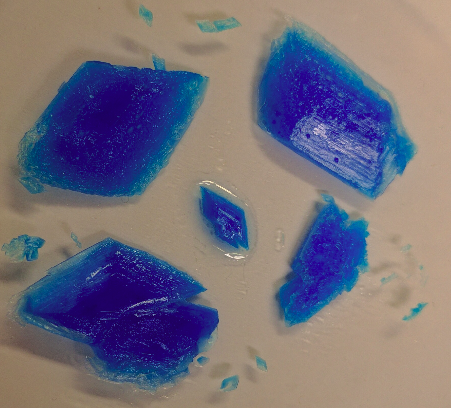
\includegraphics[scale=0.4, center]{Graphiken/Versuchsanordnungen/Kristalle.png} 
      \caption[synthetisierte Kristalle, Quelle: Autor]{Kristalle nach abgeschlossenem Trockenvorgang}
      \label{fig:Kristalle}
    \end{figure}
      
    \subsection{Weitere Berechnungen bzw. Erklärungen} \label{sec:Berechneungenweiter}
    
      Wie bereits in \ref{sec:MotivationKupfer} angemerkt, löst sich Kupfer nicht in \ch{HCl}. Dies ist darauf zurückzuführen, dass \ch{HCl} kein Oxidationsmittel wie beispielsweise \ch{HNO3} oder \ch{H2SO4} ist. Begründen kann man dies durch Anwenden der Nernstgleicchung auf die entsprechende (theoretische) Lösereaktion mit Salzsäure.
      
      \begin{reaction}
        Cu\sld{} + 2 H\pch\aq{} -> Cu\pch[2]\aq{} + H2\gas \label{rec:LosenCuHCl}
      \end{reaction}
      
      Das Standardpotential dieser Reaktion lautet wie folgt: \ElPot[superscript=0](){-0.34}. Damit läuft die Reaktion bei Standardbedingungen nicht ab. Es verbleibt zu zeigen, dass man auch durch Konzentrationsänderungen die Reaktion nicht erzwingen kann. Dazu wird die Nernstgleichung formuliert ($a_{\ch{Cu\sld}} = 1$!).
      
      \begin{equation}
        \ElPot*[](){} = \ElPot*[superscript=0](){-0.34} - \frac{R*T}{z*F} * \ln {\frac{c_{\ch{Cu\pch[2]\aq}}*p_{\ch{H2\gas}}}{c_{\ch{H\pch\aq}}^2}} \label{eq:NernsteinsCu}
      \end{equation}
      
      Zu Beginn der Reaktion ist kein \ch{Cu\pch[2]\aq} und \ch{H2\gas} vorhanden, wir betrachten somit den folgenden Grenzfall.
      
      \begin{equation}
        \lim_{c_{\ch{Cu\pch[2]}} \to 0} \ElPot*[](){} = \lim_{p_{\ch{H2\gas}} \to 0} \ElPot*[](){} = \infty
      \end{equation}  
      
      Damit läuft die Reaktion zu Beginn theoretisch freiwillig  und unendlich schnell ab\footnote{der Grenzfall ist somit physikalisch zweifelhaft und wird hier nur zur Veranschaulichung herangezogen}, aber sobald sich etwas an \ch{Cu\pch[2]\aq{}} und \ch{H2\gas} gebildet hat, nimmt das Potential schnell ab und kann vereinfachend nach \eqref{eq:NernstzweiCu} berechnet werden. Setzt man in \eqref{eq:NernstzweiCu} die Werte für Standardbedingungen ($T=\SI[mode=text]{25}{\degreeCelsius}$) ein und betrachtet eine konzentrierte \ch{HCl} ($c_{\ch{H\pch}} \approx \SI[mode=text]{12.5}{M}$), ergibt sich für das Potential: $\ElPot*[](){} = \SI[mode=text]{-0.28}{\volt}$. Die Reaktion läuft also selbst bei Verwendung von konzentrierter Salzsäure nicht ab. 
      
      \begin{equation}
        \ElPot*[](){} = \ElPot*[superscript=0](){-0.34} - \frac{R*T}{z*F} * \ln {\frac{1}{c_{\ch{H\pch\aq}}^2}} \label{eq:NernstzweiCu}
      \end{equation}
      
      Grundsätzlich ist zu beachten, dass mathematisch betrachtet, die einzelnen Variablen in \eqref{eq:NernsteinsCu} so variiert werden können, dass $\ElPot*[](){-0.34} > 0$ wird und die Reaktion damit freiwillig abläuft. Da man dazu aber beispielsweise sehr große Konzentrationen der Salzsäure zulassen müsste, sind die meisten dieser Betrachtungen physikalisch sinnlos. 
      
      Die obige Argumentation beweist, dass selbst konzentrierte Salzsäure elementares Kupfer nicht lösen kann, da ihr ein oxidierendes Anion fehlt. 
      
  \pagebreak
  
  \section{Versilbern von Glas}
  
    \subsection{Theoretische Grundlagen}
      
      \subsubsection{Motivation}
      
        Glucose ist ein Aldehyd, das zur Carbonsäure oxidiert werden kann. Ein geeignetes Oxidationsmittel sind z. B.  Silberionen, die zu elementaren Silber reduziert werden. Die zugehörigen Reaktionsgleichungen werden unten angeführt. Ammoniak muss deswegen zugegeben werden, damit das Silber durch Bildung eines Komplexes in Lösung geht, da dieses mit der Natronlauge wie beschrieben einen unlöslichen, braunen Niederschlag bildet. Anstatt die Formel für die komplette Glucose anzuführen, wird nur die Aldehydfunktion betrachtet.
        
        \begin{reaction}
          RCHO\aq{} + 2 [Ag(NH3)2]\pch\aq{} + 2 OH\mch\aq -> RCOOH\aq{} + 2 Ag\sld{} + 4 NH3\aq{} + H2O \\
        \end{reaction}
        
        \begin{reaction}
          2 AgNO3\aq{} + 2 NaOH\aq{} -> Ag2O\sld{} + 2 NaNO3\aq{} + H2O\\
        \end{reaction}
        
        \begin{reaction}
          Ag2O\sld{} + 4 NH3\sld{} + H2O -> 2 [Ag(NH3)2]\pch\aq{} + 2 OH\mch\aq \\
        \end{reaction}
        
        \begin{reactions}
          $\sum :$ RCHO\aq{} + 2 Ag\pch\aq{} + 2 OH\mch\aq{} -> RCOOH\aq{} + 2 Ag\sld{} + H2O
        \end{reactions} 
        
        Die angegebenen Reaktionen gelten auch für den sogenannten Tollens' Test in der Analytik zur Identifikation von Aldehyden \cite{Tollenstest}. \\
        
        Die Entstehung eines Silberspiegels an der Glaswand kann wie folgt erklärt werden: Silber lagert sich an der Glaswand an, da Glas an der Oberfläche freie, saure \ch{OH}-Gruppen besitzt. An diesen kann \ch{H\pch} gegen \ch{Ag\pch} ausgetauscht werden (Kationentauscher). Die eingelagerten \ch{Ag\pch} werden reduziert und bilden Anlagerungspunkte für in Lösung befindliches \ch{Ag}.  Es entsteht ein Silberspiegel.
      
      \subsubsection{Ziel des Experiments}
      
        Einem Zentrifugenröhrchen einen lebenslänglichen Silberspiegel zu verpassen.
    
    \subsection{Experimenteller Teil}
    
      \subsubsection{Verwendete Materialien}
        
        \begin{table}[H]
          \centering
          \caption[Materialienliste Versilber von Glas, Quelle: Autor]{Auflistung der verwendeten Geräte und Chemikalien}
          \label{tab:MaterialienSilberspiegel}
        
          \begin{tabular}{@{}ll|p{8cm}l@{}}
            \toprule
              Geräte & Hersteller & Chemikalie & bezogen von \\ \midrule
              Zentrifugenröhrchen &  & Lösung 1: \SI[mode=text]{13}{\gram} Zucker und \SI[mode=text]{1.3}{\gram} Traubenzucker auf \SI[mode=text]{200}{\milli\liter} \ch{H2O} & Vorrat \\
              Pasteur-Pipette &  & Lösung 2: \SI[mode=text]{2.7}{\gram} \ch{AgNO3} auf \SI[mode=text]{80}{\milli\liter} \ch{H2O} &  \\
              \SI[mode=text]{10}{\milli\liter} Messzylinder & DURAN & Lösung 3: \SI[mode=text]{2}{\gram} \ch{NaOH} auf \SI[mode=text]{80}{\milli\liter} \ch{H2O} &  \\
               &  & Lösung 4: \SI[mode=text]{10}{\gram} Natriumcitrat auf \SI[mode=text]{100}{\milli\liter} \ch{H2O} &  \\
               &  & Lösung 5: Lösung 2 und 3 wurden im Verhältnis 1:1 (V/V) gemischt, der braune \ch{Ag2O} Niederschlag wurde durch tropfenweise Zugabe von \ch{NH3} gelöst & Vorrat \\
               &  & Lösung 6: Lösung 1 und 5 wurden im Verhältnis 1:1 (V/V) gemischt &  \\ \bottomrule
          \end{tabular}
        \end{table}
      
      \subsubsection{Versuchsdurchführung}
        
        Die Lösungen 1 und 5 waren aus Zeitgründen bereits wie in Tabelle \ref{tab:MaterialienSilberspiegel} beschrieben vorbereitet. Es musste nur mehr Lösung 6 wie angegeben hergestellt werden. Dazu wurde ein \SI[mode=text]{10}{\milli\liter} Messzylinder verwendet. Die hergestellte Lösung wurde in ein mit deionisiertem Wasser ausgewaschenes Zentrifugenröhrchen transferiert. Nach ca. zwei Stunden hatte sich ein schöner Silberspiegel gebildet. Die Lösung wurde entfernt und im Schwermetallabfall entsorgt. Der Silberspiegel wurde mit deionisiertem Wasser gewaschen, um ihn beständiger zu machen.
      
    \subsection{Ergebnisse und Diskussion}
      
      Die entstandene Silberschicht im Zentrifugenröhrchen war nicht ganz so homogen und gleichmäßig wie erwartet. Auf einer Seite hatte sich ein glänzender Spiegel gebildet, auf der anderen Seite hingegen war dieser eher matt und brüchig. Beim Waschen mit Wasser lösten sich Teile von dieser Seite herunter. Außerdem hatte sich im unteren Teil des Zentrifugenröhrchens kein Silberspiegel gebildet. 
      
      Im Folgenden wird eine kurze Fehleranalyse getätigt. Die Lösung wurde zu Beginn nicht gut genug durchmischt, was eine ungleichmäßige Verteilung der Lösungen zur Folge hatte und erklärt, dass sich im unteren Teil des Zentrifugenröhrchens kein Silberspiegel ausbildete. Der brüchige Silberspiegel auf einer Seite kann durch unzureichende Reinigung des Zentrifugenröhrchens erklärt werden. Grundsätzlich könnte man eine dickere Silberschicht durch eine längere Wartezeit statt den zwei Stunden erreichen. In diesem Fall hätte es aber eher nicht dazu geführt, dass der Silberspiegel sich hätte besser und schöner ausbilden können. 
      
      Folgende Verbesserungen werden für eine erneute Durchführung vorgeschlagen:
      
      \begin{itemize}
        \item das Zentrifugenröhrchen besser reinigen
        \item die Lösung zu Beginn besser durchmischen
      \end{itemize}
  
  \pagebreak
  
  \section{Verzinken von Münzen sowie Bilden einer Messinglegierung}
  
    \subsection{Theoretische Grundlagen}
      
      \subsubsection{Motivation}
        
        Das scheinbare Vergolden, also das Vortäuschen von Gold wo keines ist, war eines der wichtigsten Ziele der Alchemisten. Messing ist eine gold-glänzende Legierung und eignet sich dazu also vortrefflich. Um eine solche Legierung herzustellen, wird auf einer Kupferschicht elementares Zink abgeschieden und dieses anschließend kurz erhitzt. 
        
        Die beim Verzinken ablaufenden Reaktionen werden im Folgenden oberflächlich beschrieben. Elementares Zink löst sich in einer alkalischen Lösung wie in \ref{rec:Zink} beschrieben. 
        
        \begin{reaction}
          Zn\sld{} + 2 OH\mch\aq{} + 2 H2O -> [Zn(OH)4]\mch[2]\aq{} + H2\gas \label{rec:Zink}
        \end{reaction}
        
        Das gebildete Zinkat kann nun reduziert werden, wobei Untersuchungen ergeben haben, dass dies an der Kupferoberfläche leichter geschieht wie an der Zinkoberfläche \cite{TheGoldenPenny}. Die Subskripte in \ref{rec:Anlagerung} bezeichnen die Oberfläche, an der die Anlagerung bzw. Ablöse der jeweiligen Zink-Spezies erfolgt.
        
        \begin{reaction}
          Zn$_{Zn}$ + [Zn(OH)4]\mch[2]\aq{} -> [Zn(OH)4]\mch[2]\aq{} + Zn$_{Cu}$ \label{rec:Anlagerung}
        \end{reaction}
        
        Bei hohen Temperaturen erfolgt der Einbau von Zink in das Kupfer schneller, weswegen sich die entsprechende Messing-Legierung erst nach dem Erhitzen ausbildet. Genaue thermodynamische und elektrochemische Begründungen können \cite{TheGoldenPenny} entnommen werden.
        
      \subsubsection{Ziel des Experiments}
        
        Das Ziel dieses Experiments ist, Kupfermünzen zu verzinken und anschließend durch Erhitzen eine Messing Legierung zu bilden.         
    
    \subsection{Experimenteller Teil}
    
      \subsubsection{Verwendete Materialien}
      
        \begin{table}[H]
          \centering
          \caption[Materialienliste Verzinken von Münzen, Quelle: Autor]{Auflistung der verwendeten Geräte und Chemikalien}
          \label{tab:MaterialienSilberspiegel}
        
          \begin{tabular}{@{}ll|ll@{}}
            \toprule
              Geräte & Hersteller & Chemikalie & Hersteller \\ \midrule
              2 \SI[mode=text]{500}{\milli\liter} Bechergläser & DURAN & \SI[mode=text]{18}{\gram} \ch{NaOH\sld}-Plätzchen & Vorrat \\
              \SI[mode=text]{250}{\milli\liter} Becherglas & DURAN & Zinkpulver & Vorrat \\
              Bunsenbrenner &  & Ethanol & Vorrat \\
              Dreifuß &  & \SI[mode=text]{14}{\percent}-ige (w/w) \ch{HNO3} & Vorrat \\
              Kupfermünzen &  & deionisiertes Wasser & Labor \\
              Tiegelzange &  &  &  \\ 
              große Kristallisierschale &  &  &  \\ \bottomrule
          \end{tabular}
        \end{table}
        
      \subsubsection{Versuchsdurchführung}
        
        Zuerst wurde eine alkalische Zinklösung hergestellt. Dazu wurden in einem \SI[mode=text]{500}{\milli\liter} Becherglas \SI[mode=text]{50}{\milli\liter} deionisiertes Wasser vorgelegt, vorsichtig \SI[mode=text]{18}{\gram} \ch{NaOH\sld} hinzugegeben und gelöst. Aufgrund des exothermen Lösevorgangs der \ch{NaOH} erwärmte sich die Lösung. Nachdem die \ch{NaOH}-Plätzchen komplett gelöst waren, wurde unter Schwenken über dem Bunsenbrenner bis zum Sieden erhitzt. Anschließend wurden \SI[mode=text]{6}{\gram} zerstoßenes Zinkpulver hinzugegeben. Die  heterogene Lösung wurde für weitere \SI[mode=text]{3}{\minute} unter Schwenken erhitzt. 
        
        Währenddessen wurden in einem \SI[mode=text]{500}{\milli\liter} Becherglas \SI[mode=text]{100}{\milli\liter} Ethanol auf ca. \SI[mode=text]{60}{\degreeCelsius} erhitzt. In dieser Lösung wurden die zu versilbernden Cent-Stücke für ca. \SI[mode=text]{2}{\minute} geschwenkt, um sie zu entfetten. Um eine Magnetisierung und daraus resultierende schlechtere Handhabung zu vermeiden, wurde auf Magnetrührer sowie Rührfisch verzichtet. Diese Utensilien wurden auch im Folgenden nicht mehr verwendet. Das Ethanol wurde abdekantiert und in das Becherglas wurden \SI[mode=text]{100}{\milli\liter} einer \SI[mode=text]{14}{\percent}-igen (w/w) \ch{HNO3} gegeben. Das Becherglas wurde nun wieder für \SI[mode=text]{2}{\minute} geschwenkt (bei Raumtemperatur). Nach dem Abdekantieren der \ch{HNO3} wurden die Münzen mit deionisiertem Wasser kurz gespült, auf ein Papiertuch gegeben\footnote{eine Berührung mit dem Fett der Finger wurde vermieden} und vorsichtig in die zu Beginn vorbereitete, heiße Zinksuspension transferiert. Dabei wurde darauf geachtet, nicht zuviele Münzen in das Becherglas zu geben, um die Kontaktoberfläche der Münzen untereinander so gering wie möglich zu halten. Die ca. \SI[mode=text]{60}{\degreeCelsius} heiße Lösung wurde für ca. \SI[mode=text]{4}{\minute} geschwenkt, bis sich auf den Münzen eine schöne Zinkschicht gebildet hatte. Die Münzen wurden in ein mit deionisiertem Wasser gefülltes \SI[mode=text]{100}{\milli\liter} Becherglas transferiert und mehrmals gewaschen. Alle Zinkabfälle bzw. mit Zink behaftete Papiertücher, ... wurden in einer großen Kristallisierschale gesammelt und im Abzug mit \ch{HCl} versetzt, damit sich das elementare Zink auflöst\footnote{angefeuchtetes Zink kann mit Papier unmittelbar zum Brennen anfangen}.
        
        Ein Teil der versilberten Münzen wurde mit einer Tiegelzange bei mittlerer Hitze über eine Bunsenbrennerflamme gehalten. Es wurde gewartet, bis sich eine goldene Messingschicht ausbildete. Die Münzen wurden kurz in einem mit Wasser gefüllten \SI[mode=text]{100}{\milli\liter} Becherglas abgekühlt.
      
    \subsection{Ergebnisse und Diskussion}
      
      Sowohl die Anlagerung von Zink an die Münzen als auch das Ausbilden der Messingschicht funktionierten sehr gut. Die Zinkschicht war bei allen Münzen an allen Stellen schön gleichmäßig vorhanden und die Messingschicht bildete sich bei allen Münzen problemlos. 
      
      
    
  \pagebreak
  
  \listofreactions
  \printbibliography[title=Literaturverzeichnis]
  \listoffigures
  \listoftables
  
\end{document}
